\toclesssection{Cache Efficiency}

\toclesssubsection{Introduction}

\begin{frame}{Cache Efficiency}{Introduction}
  \textbf{Background:}
  \begin{itemize}
    \item<2->
      Up to now we always counted the {\color{MainA}number of operations}
    \item<2->
      Assuming this is a good measure for the runtime of an algorithm/tool
    \item<3->
      Today we will see examples where this is not suitable
  \end{itemize}
\end{frame}

%-------------------------------------------------------------------------------

\begin{frame}{Cache Efficiency}{Introduction}
  \textbf{Example:}
  \begin{itemize}
    \item
      We sum up all elements of an array {\color{MainA}$a$} of size
      {\color{MainA}$n$} in $\ldots$
    \begin{itemize}
      \item
        natural order:
        \begin{displaymath}
          {\color{MainA}\mathrm{sum}(a)} =
          {\color{MainA}a[1]} +
          {\color{MainA}a[2]} +
          \dots +
          {\color{MainA}a[n]}
        \end{displaymath}
      \item
        random order:
        \begin{displaymath}
          {\color{MainA}\mathrm{sum}(a)} =
          {\color{MainA}a[21]} +
          {\color{MainA}a[5]} +
          \dots +
          {\color{MainA}a[8]}
        \end{displaymath}
    \end{itemize}
  \end{itemize}
\end{frame}

%-------------------------------------------------------------------------------

\codeslide{python}{
\begin{frame}{Cache Efficiency}{Linear Order - Python}
  \textbf{Python:}
  \lstinputlisting[
    language=Python,
    basicstyle=\small,
    tabsize=4,
    style={python-idle-code},
    escapechar={@},
    emph={init},
    emphstyle=\color{blue}
  ]{Code/Caching/CacheLinear_Part1.py}
\end{frame}

%-------------------------------------------------------------------------------

\begin{frame}{Cache Efficiency}{Linear Order - Python}
  \textbf{Python:}
  \lstinputlisting[
    language=Python,
    basicstyle=\small,
    tabsize=4,
    style={python-idle-code},
    escapechar={@},
    emph={run},
    emphstyle=\color{blue}
  ]{Code/Caching/CacheLinear_Part2.py}
\end{frame}
}

%TODO: Implement algorithm in Java / C++
%%-------------------------------------------------------------------------------
%
%\codeslide{java}{
%\begin{frame}{Cache Efficiency}{Linear Order - Java}
%  \textbf{Java:}
%  \lstinputlisting[
%    language=Java,
%    basicstyle=\small,
%    tabsize=4,
%    style={java-eclipse-code},
%    escapechar={@},
%    emph={words},
%    emphstyle=\color{java_variable}
%  ]{Code/Caching/CacheLinear.java}
%\end{frame}
%}
%
%%-------------------------------------------------------------------------------
%
%\codeslide{cpp}{
%\begin{frame}{Cache Efficiency}{Linear Order - C++}
%  \textbf{C++:}
%  \lstinputlisting[
%    language=C++,
%    basicstyle=\small,
%    tabsize=4,
%    style={cpp-eclipse-code},
%    morekeywords={endl},
%    escapechar={@}
%  ]{Code/Caching/CacheLinear.cpp}
%\end{frame}
%}

%-------------------------------------------------------------------------------

\begin{frame}{Cache Efficiency}{Linear Order}
  \begin{figure}
    \begin{center}
      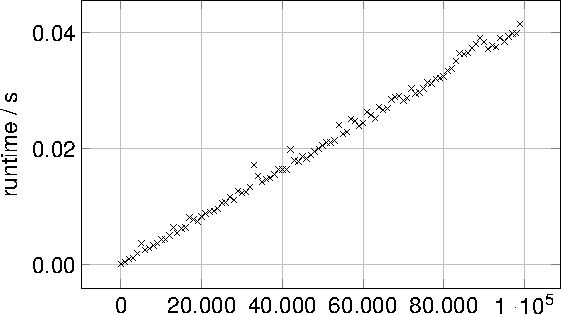
\includegraphics[width=0.7\textwidth]{Images/Caching/sumlinear-plot.pdf}
    \end{center}
    \caption{summing elements in linear order}
    \label{fig:caching:sum_linear_order}
  \end{figure}
\end{frame}

%-------------------------------------------------------------------------------

\codeslide{python}{
\begin{frame}{Cache Efficiency}{Random Order - Python}
  \lstinputlisting[
    language=Python,
    basicstyle=\small,
    tabsize=4,
    style={python-idle-code},
    escapechar={@},
    emph={init},
    emphstyle=\color{blue},
    breaklines=false
  ]{Code/Caching/CacheRandom.py}
\end{frame}
}

%TODO: Implement algorithm in Java / C++
%%-------------------------------------------------------------------------------
%
%\codeslide{java}{
%\begin{frame}{Cache Efficiency}{Random Order - Java}
%  \textbf{Java:}
%  \lstinputlisting[
%    language=Java,
%    basicstyle=\small,
%    tabsize=4,
%    style={java-eclipse-code},
%    escapechar={@},
%    emph={words},
%    emphstyle=\color{java_variable}
%  ]{Code/Caching/CacheLinear.java}
%\end{frame}
%}
%
%%-------------------------------------------------------------------------------
%
%\codeslide{cpp}{
%\begin{frame}{Cache Efficiency}{Random Order - C++}
%  \textbf{C++:}
%  \lstinputlisting[
%    language=C++,
%    basicstyle=\small,
%    tabsize=4,
%    style={cpp-eclipse-code},
%    morekeywords={endl},
%    escapechar={@}
%  ]{Code/Caching/CacheLinear.cpp}
%\end{frame}
%}

%-------------------------------------------------------------------------------

\begin{frame}{Cache Efficiency}{Random Order}
  \begin{figure}
    \begin{center}
      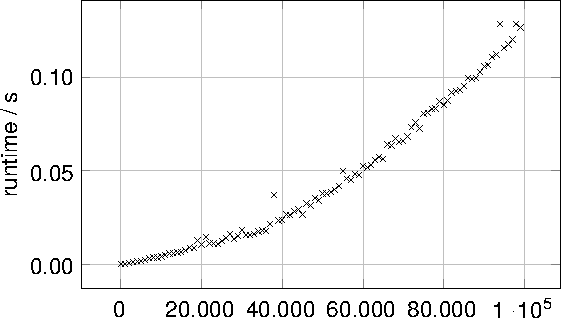
\includegraphics[width=0.7\textwidth]{Images/Caching/sumrandom-plot.pdf}
    \end{center}
    \caption{summing elements in random order}
    \label{fig:caching:sum_random_order}
  \end{figure}
\end{frame}

%-------------------------------------------------------------------------------

\begin{frame}{Cache Efficiency}{Algorithm Comparision}
  \textbf{Conclusion:}
  \begin{itemize}
    \item<2->
      The number of operations is identical for both algorithms
    \item<3->
      Accessing elements in random order takes a lot longer (factor 10)
      \onslide<3-| handout: 0>{{\color{MainA}Why?}\\}
    \item<3->
      The costs in terms of memory access are very different
  \end{itemize}
\end{frame}

%-------------------------------------------------------------------------------

\subsection{Cache Organization}

\begin{frame}{Cache Efficiency}{CPU Cache}
  \vspace{-1.5em}
  \begin{figure}
    \begin{adjustbox}{width=\linewidth}
      \begin{tikzpicture}[
  cell/.style={
  }, cell_active/.style={
    cell,
    fill=Hell-Gruen,
  }, cell_text/.style={
    color=black,
    font=\Large
  }, block/.style={
    draw=black
  }, block_active/.style={
    block,
    fill=Hell-Blau
  }
]%
% position x / y, block active, cell data {n x [cell active]}
\foreach \x/\y/\a/\d in {%
  0/0/0/{0,0,0,0,0,0,0,0},%
  5/0/0/{0,0,0,0,0,0,0,0},%
  10/0/1/{0,0,0,0,0,1,0,0},%
  15/0/0/{0,0,0,0,0,0,0,0},%
  20/0/0/{0,0,0,0,0,0,0,0},%
  0/-3/0/{0,0,0,0,0,0,0,0},%
  5/-3/1/{0,0,0,0,0,1,0,0},%
  10/-3/0/{0,0,0,0,0,0,0,0},%
  0/-6/0/{0,1,0,0,0,0,0,0}%
}{%
  % draw block
  \ifnum \a>0
    \draw[block_active] (\x, \y) rectangle ++(5.0, 1.0);
  \else
    \draw[block] (\x, \y) rectangle ++(5.0, 1.0);
  \fi
  
  % draw cells
  \foreach \ca [count=\index] in \d {
    \ifnum \ca>0
      \draw[cell_active]
        (\x + 0.625*\index - 0.625, \y) rectangle ++(0.625, 1.0);
    \fi
    
    \node[cell_text] at (\x + 0.625*\index - 0.3125, \y + 0.5) {$0$};
  }
}

% labels
\node[font=\Huge, anchor=east] at (-0.25, 0.5) {Memory};
\node[font=\Huge, anchor=east] at (-0.25, -2.5) {Cache};
\node[font=\Huge, anchor=east] at (-0.25, -5.5) {Register};

% arrows
\draw[<->, color=red, ultra thick, line width=0.25em]
  (10 + 3.125 + 0.3125, -0.25) to
  node[cell_text, color=red, fill=white, midway, font=\Huge, sloped] {slow}
  (5 + 3.125 + 0.3125, -1.75);
\draw[<->, color=Mittel-Gruen, ultra thick, line width=0.25em]
  (5 + 3.125 + 0.3125, -3.25) to
  node[cell_text, color=Mittel-Gruen, fill=white, midway, font=\Huge, sloped]
    {fast}
  (0.625 + 0.3125, -4.75);
\end{tikzpicture}
    \end{adjustbox}
    \label{fig:caching:cache_hirarchy}
  \end{figure}
  \onslide<2->
  \textbf{Principle / organization:}
  \begin{itemize}
    \item<3->
      Accessing one byte of the main memory takes
      $\approx\SI{100}{\nano\second}$
    \item<4->
      Accessing one byte of (L1-)cache takes
      $\approx\SI{1}{\nano\second}$
    \item<5->
      Accessing one or more byte/s of main memory loads a whole
      block $\approx\SI{100}{\byte}$ into the cache
    \item<6->
      As long as this block is in the cache, it is not neccessary to
      access the memory for bytes of this block
  \end{itemize}
\end{frame}

%-------------------------------------------------------------------------------

\begin{frame}{Cache Efficiency}{CPU Cache}
  \vspace{-1.5em}
  \begin{figure}
    \begin{adjustbox}{width=\linewidth}
      \begin{tikzpicture}[
  cell/.style={
  }, cell_active/.style={
    cell,
    fill=Hell-Gruen,
  }, cell_text/.style={
    color=black,
    font=\Large
  }, block/.style={
    draw=black
  }, block_active/.style={
    block,
    fill=Hell-Blau
  }
]%
% position x / y, block active, cell data {n x [cell active]}
\foreach \x/\y/\a/\d in {%
  0/0/0/{0,0,0,0,0,0,0,0},%
  5/0/0/{0,0,0,0,0,0,0,0},%
  10/0/1/{0,0,0,0,0,1,0,0},%
  15/0/0/{0,0,0,0,0,0,0,0},%
  20/0/0/{0,0,0,0,0,0,0,0},%
  0/-3/0/{0,0,0,0,0,0,0,0},%
  5/-3/1/{0,0,0,0,0,1,0,0},%
  10/-3/0/{0,0,0,0,0,0,0,0},%
  0/-6/0/{0,1,0,0,0,0,0,0}%
}{%
  % draw block
  \ifnum \a>0
    \draw[block_active] (\x, \y) rectangle ++(5.0, 1.0);
  \else
    \draw[block] (\x, \y) rectangle ++(5.0, 1.0);
  \fi
  
  % draw cells
  \foreach \ca [count=\index] in \d {
    \ifnum \ca>0
      \draw[cell_active]
        (\x + 0.625*\index - 0.625, \y) rectangle ++(0.625, 1.0);
    \fi
    
    \node[cell_text] at (\x + 0.625*\index - 0.3125, \y + 0.5) {$0$};
  }
}

% labels
\node[font=\Huge, anchor=east] at (-0.25, 0.5) {Memory};
\node[font=\Huge, anchor=east] at (-0.25, -2.5) {Cache};
\node[font=\Huge, anchor=east] at (-0.25, -5.5) {Register};

% arrows
\draw[<->, color=red, ultra thick, line width=0.25em]
  (10 + 3.125 + 0.3125, -0.25) to
  node[cell_text, color=red, fill=white, midway, font=\Huge, sloped] {slow}
  (5 + 3.125 + 0.3125, -1.75);
\draw[<->, color=Mittel-Gruen, ultra thick, line width=0.25em]
  (5 + 3.125 + 0.3125, -3.25) to
  node[cell_text, color=Mittel-Gruen, fill=white, midway, font=\Huge, sloped]
    {fast}
  (0.625 + 0.3125, -4.75);
\end{tikzpicture}
    \end{adjustbox}
    \label{fig:caching:cache_hirarchy2}
  \end{figure}
  \vspace{-0.3cm}
  \onslide<2->
  \textbf{Cache organization:}
  \begin{itemize}
    \item<3->
      The (L1-)cache can hold multiple memory blocks
      \begin{itemize}
        \item<4->
          Cache lines $\approx\SI{100}{\kilo\byte}$
        \end{itemize}
    \item<5->
      If the capacity is reached unused blocks are discarded
      \begin{itemize}
        \item<6->
          {\color{MainA}Least recently used (LRU)}
        \item<7->
          {\color{MainA}Least frequently used (LFU)}
        \item<8->
          {\color{MainA}First in first out (FIFO)}
      \end{itemize}
      \item<9-> Details of discarding not discussed today
  \end{itemize}
\end{frame}

%-------------------------------------------------------------------------------

\begin{frame}{Cache Efficiency}{Block Operations}
  \vspace{-2.0em}
  \begin{figure}%
    \begin{adjustbox}{width=\linewidth}%
      \begin{tikzpicture}[
  cell/.style={
  }, cell_active/.style={
    cell,
    fill=Hell-Gruen,
  }, cell_text/.style={
    color=black,
    font=\Large
  }, block/.style={
    draw=black
  }, block_active/.style={
    block,
    fill=Hell-Blau
  }
]%
% position x / y, block active, cell data {n x [cell active]}
\foreach \x/\y/\a/\d in {%
  0/0/0/{0,0,0,0,0,0,0,0},%
  5/0/0/{0,0,0,0,0,0,0,0},%
  10/0/1/{0,0,0,0,0,1,0,0},%
  15/0/0/{0,0,0,0,0,0,0,0},%
  20/0/0/{0,0,0,0,0,0,0,0},%
  0/-3/0/{0,0,0,0,0,0,0,0},%
  5/-3/1/{0,0,0,0,0,1,0,0},%
  10/-3/0/{0,0,0,0,0,0,0,0}%
}{%
  % draw block
  \ifnum \a>0
    \draw[block_active] (\x, \y) rectangle ++(5.0, 1.0);
  \else
    \draw[block] (\x, \y) rectangle ++(5.0, 1.0);
  \fi
  
  % draw cells
  \foreach \ca [count=\index] in \d {
    \ifnum \ca>0
      \draw[cell_active]
        (\x + 0.625*\index - 0.625, \y) rectangle ++(0.625, 1.0);
    \fi
    
    \node[cell_text] at (\x + 0.625*\index - 0.3125, \y + 0.5) {$0$};
  }
}

% labels
\node[font=\Huge, anchor=east] at (-0.25, 0.5) {Memory};
\node[font=\Huge, anchor=east] at (-0.25, -2.5) {Cache};

% upper brace (block)
\draw[
  line width=0.25em,
  decoration={brace, raise=0.75em, amplitude=1.0em},
  decorate
] (0, 1) --
    node[midway, yshift=4em, font=\Huge]
    {{\color{Mittel-Blau}$B$} bytes}
  (5, 1);

% lower brace (cache)
\draw[
  line width=0.25em,
  decoration={brace, raise=0.75em, amplitude=1.0em, mirror},
  decorate
] (0, -3) --
    node[midway, yshift=-4em, color=Mittel-Blau, font=\Huge]
    {{\color{Mittel-Blau}$M$} bytes = {\color{Mittel-Blau}$M/B$} blocks}
  (15, -3);
\end{tikzpicture}%
    \end{adjustbox}%
    \label{fig:caching:cache_quanting}
  \end{figure}%
  \textbf{Terminology:}
  \begin{itemize}
    \item<2->
      The system consists of slow and fast memory 
    \item<3->
      The {\color{MainA}slow memory} is divided in
      {\color{MainA}blocks of size $B$}
    \item<4->
      The {\color{MainA}fast cache} has size $M$ an can store $M/B$
      blocks
    \item<5->
      If data is not in fast memory, the corresponding block is loaded into the {\color{MainA}cache}
  \end{itemize}
\end{frame}

%-------------------------------------------------------------------------------

\begin{frame}{Cache Efficiency}{Block Operations}
  \vspace{-2.0em}
  \begin{figure}%
    \begin{adjustbox}{width=\linewidth}%
      \begin{tikzpicture}[
  cell/.style={
  }, cell_active/.style={
    cell,
    fill=Hell-Gruen,
  }, cell_text/.style={
    color=black,
    font=\Large
  }, block/.style={
    draw=black
  }, block_active/.style={
    block,
    fill=Hell-Blau
  }
]%
% position x / y, block active, cell data {n x [cell active]}
\foreach \x/\y/\a/\d in {%
  0/0/0/{0,0,0,0,0,0,0,0},%
  5/0/0/{0,0,0,0,0,0,0,0},%
  10/0/1/{0,0,0,0,0,1,0,0},%
  15/0/0/{0,0,0,0,0,0,0,0},%
  20/0/0/{0,0,0,0,0,0,0,0},%
  0/-3/0/{0,0,0,0,0,0,0,0},%
  5/-3/1/{0,0,0,0,0,1,0,0},%
  10/-3/0/{0,0,0,0,0,0,0,0}%
}{%
  % draw block
  \ifnum \a>0
    \draw[block_active] (\x, \y) rectangle ++(5.0, 1.0);
  \else
    \draw[block] (\x, \y) rectangle ++(5.0, 1.0);
  \fi
  
  % draw cells
  \foreach \ca [count=\index] in \d {
    \ifnum \ca>0
      \draw[cell_active]
        (\x + 0.625*\index - 0.625, \y) rectangle ++(0.625, 1.0);
    \fi
    
    \node[cell_text] at (\x + 0.625*\index - 0.3125, \y + 0.5) {$0$};
  }
}

% labels
\node[font=\Huge, anchor=east] at (-0.25, 0.5) {Memory};
\node[font=\Huge, anchor=east] at (-0.25, -2.5) {Cache};

% upper brace (block)
\draw[
  line width=0.25em,
  decoration={brace, raise=0.75em, amplitude=1.0em},
  decorate
] (0, 1) --
    node[midway, yshift=4em, font=\Huge]
    {{\color{Mittel-Blau}$B$} bytes}
  (5, 1);

% lower brace (cache)
\draw[
  line width=0.25em,
  decoration={brace, raise=0.75em, amplitude=1.0em, mirror},
  decorate
] (0, -3) --
    node[midway, yshift=-4em, color=Mittel-Blau, font=\Huge]
    {{\color{Mittel-Blau}$M$} bytes = {\color{Mittel-Blau}$M/B$} blocks}
  (15, -3);
\end{tikzpicture}%
    \end{adjustbox}%
    \label{fig:caching:cache_quanting2}
  \end{figure}%
  \textbf{Terminology:}
  \begin{itemize}
    \item<2->
      The program defines which blocks are held in the
      {\color{MainA}cache}
    \item<3->
      We use the number of {\color{MainA}block operations} as runtime
      estimation
    \item<4->
      We ignore runtime costs of cache access / management
  \end{itemize}
\end{frame}

%-------------------------------------------------------------------------------

\begin{frame}{Cache Efficiency}{Block Operations}
  \vspace{-2.0em}
  \begin{figure}%
    \begin{adjustbox}{width=\linewidth}%
      \begin{tikzpicture}[
  cell/.style={
  }, cell_active/.style={
    cell,
    fill=Hell-Gruen,
  }, cell_text/.style={
    color=black,
    font=\Large
  }, block/.style={
    draw=black
  }, block_active/.style={
    block,
    fill=Hell-Blau
  }
]%
% position x / y, block active, cell data {n x [cell active]}
\foreach \x/\y/\a/\d in {%
  0/0/0/{0,0,0,0,0,0,0,0},%
  5/0/0/{0,0,0,0,0,0,0,0},%
  10/0/1/{0,1,1,1,1,1,0,0},%
  15/0/0/{0,0,0,0,0,0,0,0},%
  20/0/0/{0,0,0,0,0,0,0,0},%
  0/-3/1/{0,0,1,0,0,0,0,0},%
  5/-3/1/{0,0,0,0,0,1,0,0},%
  10/-3/1/{0,0,1,0,0,0,0,0},%
  15/-3/1/{0,0,0,0,0,1,0,0},%
  20/-3/1/{0,1,0,0,0,0,0,0}%
}{%
  % draw block
  \ifnum \a>0
    \draw[block_active] (\x, \y) rectangle ++(5.0, 1.0);
  \else
    \draw[block] (\x, \y) rectangle ++(5.0, 1.0);
  \fi
  
  % draw cells
  \foreach \ca [count=\index] in \d {
    \ifnum \ca>0
      \draw[cell_active]
        (\x + 0.625*\index - 0.625, \y) rectangle ++(0.625, 1.0);
    \fi
    
    \node[cell_text] at (\x + 0.625*\index - 0.3125, \y + 0.5) {$0$};
  }
}

% labels
\node[font=\Huge, anchor=east] at (-0.25, 0.5) {Memory};
\node[font=\Huge, anchor=east] at (-0.25, -2.5) {Memory};
\node[font=\Huge, anchor=south] at (12.5, 1.15)
  {good locality};
\node[font=\Huge, anchor=south] at (12.5, -1.85)
  {bad locality};
\end{tikzpicture}%
    \end{adjustbox}%
    \caption{comparison good / bad locality}
    \label{fig:caching:memory_locality}
  \end{figure}%
  \textbf{Accessing the cache {\color{MainA}$B$} times:}
  \begin{itemize}
    \item
      {\color{MainA}Best case}:
      1 block operation $\rightarrow$ good locality
    \item
      {\color{MainA}Worst case}:
      {\color{MainA}$B$} block operations $\rightarrow$ bad locality
  \end{itemize}
\end{frame}

%-------------------------------------------------------------------------------

\begin{frame}{Cache Efficiency}{Block Operations}
  \textbf{Additional factors:}\\
  \begin{itemize}
    \item<2->
    The following settings change only a small constant factor in number of block operations
    \begin{itemize}
    \item<3-> Partionining of the slow memory into blocks
    \item<4-> Regardless of the block size: {\color{MainA}1 bytes} or
      {\color{MainA}4 bytes} or {\color{MainA}8 bytes}
    \end{itemize}
  \end{itemize}
  \vspace{1.0em}
  \onslide<5->
  \textbf{Note:}\\
  \begin{itemize}
    \item<6->
      If the {\color{MainA}input size} is
      {\color{MainA}smaller than $M$} we load the complete data chunk
      directly into the cache
    \item<7->
      Cache handling is only interesting when the
      {\color{MainA}input size} is
      {\color{MainA}greater than $M$}
  \end{itemize}
\end{frame}

%-------------------------------------------------------------------------------

\begin{frame}{Cache Efficiency}{Block Operations}
  \textbf{Typical values:}
  (\texttt{Intel$\copyright$ i7-4770} Haswell,
  \texttt{WD$\copyright$ Blue} $\SI{2}{\tera\byte}$)
  \begin{itemize}
    \item<2->
      CPU L1 Cache: {\color{MainA}$B = \SI{64}{\byte}$},
      {\color{MainA}$M = 4 \times (\SI{32}{\kilo\byte} + \SI{32}{\kilo\byte})$}
    \item<3->
      CPU L2 Cache: {\color{MainA}$B = \SI{64}{\byte}$}, {\color{MainA}$M = 4 \times \SI{256}{\kilo\byte}$}
    \item<4->
      CPU L3 Cache: {\color{MainA}$B = \SI{64}{\byte}$}, {\color{MainA}$M = \SI{8}{\mega\byte}$}
    \item<4->
      Disk Cache: {\color{MainA}$B = \SI{64}{\kilo\byte}$}, {\color{MainA}$M = \SI{64}{\mega\byte}$}
    \begin{itemize}
      \item<5->
        Many operating systems use free system memory as disk cache
    \end{itemize}
  \end{itemize}
\end{frame}

%-------------------------------------------------------------------------------

\begin{frame}{Cache Efficiency}{Block Operations}
  \textbf{Terminology:}
  \begin{itemize}
    \item<2->
      Block loads on CPU cache are called {\color{MainA}cache~misses}
    \item<3->
      Block operations on disk cache are called {\color{MainA}IOs}\\
      (input / output operations)
    \item<4->
      These also fall under the term {\color{MainA}cache~efficiency} or
      {\color{MainA}IO~efficiency}
  \end{itemize}
\end{frame}

%-------------------------------------------------------------------------------

\begin{frame}{Cache Efficiency}{Block Operations - Linear Order}
  \vspace{-1.0em}
  \textbf{Example 1 - Linear order:}
  \begin{itemize}
    \item<2->
      We sum up all elements in {\color{MainA}natural order}
      \begin{displaymath}
        {\color{MainA}\mathrm{sum}(a)} =
        {\color{MainA}a[1]} +
        {\color{MainA}a[2]} +
        \dots +
        {\color{MainA}a[n]}
      \end{displaymath}
    \item<3->
      The number of block operations is
      {\color{MainA}$\mathrm{ceil}\left(\frac{n}{B}\right)$}
  \end{itemize}
  \vspace{-1.0em}
  \onslide<4->
  \begin{figure}%
    \begin{adjustbox}{width=\linewidth}%
      \begin{tikzpicture}[
  cell_active/.style={
    fill=Hell-Gruen,
  }, cell_text/.style={
    color=black,
    font=\Large
  }, cell_arrow/.style={
    line width=0.25em,
    color=Mittel-Gruen
  }, block/.style={
    draw=black
  }, block_active/.style={
    block,
    fill=Hell-Blau
  }, block_arrow/.style={
    line width=0.5em,
    color=Mittel-Blau
  }
]%
% position x / y, block active, cell data {n x [cell active]}
\foreach \x/\y/\a/\d in {%
  0/0/1/{1,1,1,1,1,1,1,1},%
  5/0/1/{1,1,1,1,0,0,0,0},%
  10/0/0/{0,0,0,0,0,0,0,0},%
  15/0/0/{0,0,0,0,0,0,0,0},%
  20/0/0/{0,0,0,0,0,0,0,0}%
}{%
  % draw block
  \ifnum \a>0
    \fill[block_active] (\x, \y) rectangle ++(5.0, 1.0);
    \draw[->, block_arrow] (\x + 2.5, \y - 0.15) -- ++(0, -0.75);
  \fi
  
  % draw cells
  \foreach \ca [count=\index] in \d {
    \ifnum \ca>0
      \fill[cell_active]
        (\x + 0.625*\index - 0.625, \y) rectangle ++(0.625, 1.0);
      
      \draw[<-, cell_arrow]
        (\x + 0.625*\index - 0.3125, \y + 1.15) -- ++(0, 0.75);
    \fi
    
    \node[cell_text] at (\x + 0.625*\index - 0.3125, \y + 0.5) {$0$};
  }
  
  \draw[block] (\x, \y) rectangle ++(5.0, 1.0);
}

% labels
\node[font=\Huge, anchor=east] at (-0.25, 0.5) {Cache};
\node[font=\Huge, anchor=south, color=Mittel-Gruen] at (5, 2.15)
  {Cache Read / Write};
\node[font=\Huge, anchor=north, color=Mittel-Blau] at (5, -1.15)
  {Block Read / Write};
\end{tikzpicture}%
    \end{adjustbox}%
    \caption{good locality of sum operation}
    \label{fig:caching:memory_locality_linear}
  \end{figure}%
\end{frame}

%-------------------------------------------------------------------------------

\begin{frame}{Cache Efficiency}{Block Operations - Random Order}
  \textbf{Example 2 - Random order:}
  \begin{itemize}
    \item<2->
      We sum up all elements in {\color{MainA}random order}
      \begin{displaymath}
        {\color{MainA}\mathrm{sum}(a)} =
        {\color{MainA}a[21]} +
        {\color{MainA}a[5]} +
        \dots +
        {\color{MainA}a[8]}
      \end{displaymath}
    \item<3->
      The number of block operations is {\color{MainA}$n$} in the
      {\color{MainA}worst case}
    \item<4->
      This leads to a runtime factor difference of {\color{MainA}$B$}
  \end{itemize}
  \onslide<5->
   \vspace{-1.0em}
  \begin{figure}%
    \begin{adjustbox}{width=\linewidth}%
      \begin{tikzpicture}[
  cell_active/.style={
    fill=Hell-Gruen,
  }, cell_text/.style={
    color=black,
    font=\Large
  }, cell_arrow/.style={
    line width=0.25em,
    color=Mittel-Gruen
  }, block/.style={
    draw=black
  }, block_active/.style={
    block,
    fill=Hell-Blau
  }, block_arrow/.style={
    line width=0.5em,
    color=Mittel-Blau
  }
]%
% position x / y, block active, cell data {n x [cell active]}
\foreach \x/\y/\a/\d in {%
  0/0/1/{1,0,0,1,0,0,1,0},%
  5/0/1/{1,0,0,0,0,0,1,1},%
  10/0/1/{0,1,0,0,0,0,0,1},%
  15/0/1/{0,0,0,1,0,1,0,0},%
  20/0/1/{0,0,1,0,0,1,0,0}%
}{%
  % draw block
  \ifnum \a>0
    \fill[block_active] (\x, \y) rectangle ++(5.0, 1.0);
    \draw[->, block_arrow] (\x + 2.5, \y - 0.15) -- ++(0, -0.75);
  \fi
  
  % draw cells
  \foreach \ca [count=\index] in \d {
    \ifnum \ca>0
      \fill[cell_active]
        (\x + 0.625*\index - 0.625, \y) rectangle ++(0.625, 1.0);
      
      \draw[<-, cell_arrow]
        (\x + 0.625*\index - 0.3125, \y + 1.15) -- ++(0, 0.75);
    \fi
    
    \node[cell_text] at (\x + 0.625*\index - 0.3125, \y + 0.5) {$0$};
  }
  
  \draw[block] (\x, \y) rectangle ++(5.0, 1.0);
}

% labels
\node[font=\Huge, anchor=east] at (-0.25, 0.5) {Cache};
\node[font=\Huge, anchor=south, color=Mittel-Gruen] at (12.5, 2.15)
  {Cache Read / Write};
\node[font=\Huge, anchor=north, color=Mittel-Blau] at (12.5, -1.15)
  {Block Read / Write};
\end{tikzpicture}%
    \end{adjustbox}%
    \caption{bad locality of sum operation}
    \label{fig:caching:memory_locality_random}
  \end{figure}%
  \vspace{-1.0em}
\end{frame}

%-------------------------------------------------------------------------------

\begin{frame}{Cache Efficiency}{Block Operations}
  \textbf{Generally the factor is substantially {\color{MainA}$< B$}}
  \begin{itemize}
    \item<2->
      Even with a {\color{MainA}random order} we access 4
      neighboring bytes at once per \texttt{int} (\text{int32\_t})
    \item<3->
      The next element might already be loaded into the cache
    \item<4->
      If {\color{MainA}not $n \gg M$} this might occur with a high probability 
  \end{itemize}
\end{frame}

%-------------------------------------------------------------------------------

\begin{frame}{Cache Efficiency}{Block Operations - Quicksort}
  \textbf{Quicksort:}\\
  \begin{itemize}
    \item<2->
      \textbf{Strategy:} Divide and Conquer
    \item<3->
      Divide the data into two parts where the \enquote{left} part contains
      all values {\color{MainA}$\leq$} the values in the right part
    \item<4->
      Choose one element (e.g the first one) as
      {\color{MainA}\enquote{pivot} element}
    \item<5->
      Ideally both parts are the same size
    \item<6->
      Both parts are sorted recursively
  \end{itemize}
  \onslide<7->
  \vspace{-1em}
  \begin{figure}%
    \begin{adjustbox}{width=\linewidth}%
      \begin{tikzpicture}[
  list/.style={
    draw=black
  }, pivot/.style={
    list,
    fill=Hell-Gruen
  }, label/.style={
    color=Mittel-Blau,
    font=\huge
  }, label_pivot/.style={
    color=black,
    font=\huge
  }
]%
% upper list
\draw[list] (0, 0) rectangle ++(16, 1);
\draw[pivot] (0, 0) rectangle ++(1, 1);

\node[label_pivot] at (0.5, 0.5) {p};
\node[label] at (8.5, 0.5) {list};

% lower list
\draw[list] (0, -1.5) rectangle ++(16, 1);
\draw[pivot] (4, -1.5) rectangle ++(1, 1);

\node[label] at (2, -1) {lower list};
\node[label_pivot] at (4.5, -1) {p};
\node[label] at (10.5, -1) {upper list};
\end{tikzpicture}%
    \end{adjustbox}%
    \caption{\textit{Quicksort} with pivot element}
    \label{fig:caching:quicksort_pivot}
  \end{figure}%
\end{frame}

%-------------------------------------------------------------------------------

\begin{frame}
  \frametitle{Idea of Quicksort}
  \begin{itemize}
  \item \textbf{At start:} pivot in first position, first re-arrange list such
    that left part contains smaller and right part larger elements
  \item Do required changes \emph{in place}
  \end{itemize}
  \hspace*{1cm}\onslide<1>{\rlap{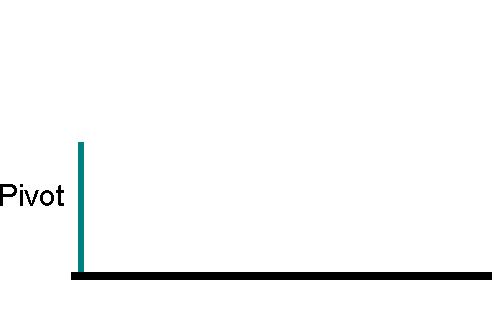
\includegraphics[width=0.55\textwidth]{Images/Caching/quicksort-idea-o1.pdf}}}%
  \onslide<2>{\rlap{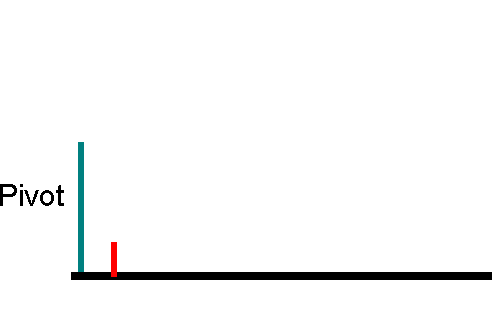
\includegraphics[width=0.55\textwidth]{Images/Caching/quicksort-idea-o2.pdf}}}%
  \onslide<3>{\rlap{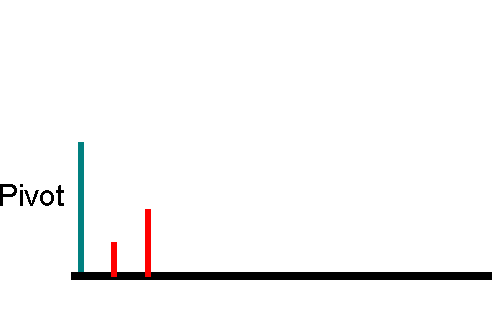
\includegraphics[width=0.55\textwidth]{Images/Caching/quicksort-idea-o3.pdf}}}%
  \onslide<4>{\rlap{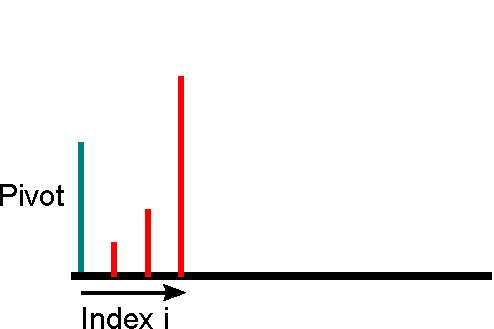
\includegraphics[width=0.55\textwidth]{Images/Caching/quicksort-idea-o4.pdf}}}%
  \onslide<5>{\rlap{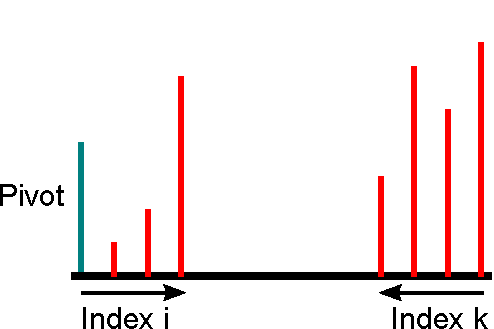
\includegraphics[width=0.55\textwidth]{Images/Caching/quicksort-idea-o5.pdf}}}%
  \onslide<6>{\rlap{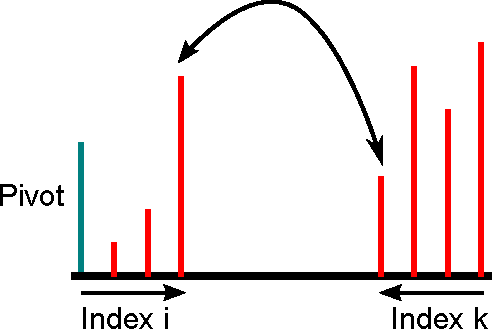
\includegraphics[width=0.55\textwidth]{Images/Caching/quicksort-idea-o6.pdf}}}%
  \onslide<7->{\rlap{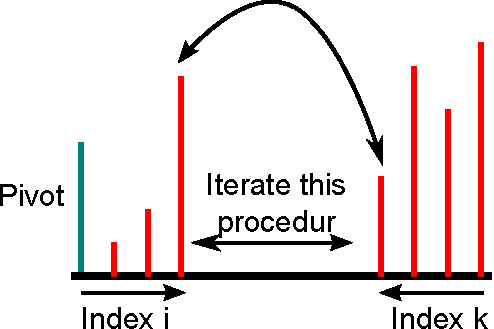
\includegraphics[width=0.55\textwidth]{Images/Caching/quicksort-idea-o7.pdf}}}%
  \begin{itemize}
  \item \textbf{End point:} $k$ is left to left-most element greater than pivot
    \begin{center}
     \textit{swap position 0 (pivot) with $k$ (smaller than pivot)}
    \end{center}
  \end{itemize}
\end{frame}

%-------------------------------------------------------------------------------

\codeslide{python}{
\begin{frame}{Cache Efficiency}{Block Operations - Quicksort - Python}
  \textbf{Python:}
  \lstinputlisting[
    language=Python,
    basicstyle=\normalsize,
    tabsize=2,
    style={python-idle-code},
    breaklines=false,
    escapechar={@},
    emph={quicksort},
    emphstyle=\color{blue}
  ]{Code/Caching/QuickSort_Part1.py}
\end{frame}

%-------------------------------------------------------------------------------

\begin{frame}{Cache Efficiency}{Block Operations - Quicksort - Python}
  \vspace{-1em}
  \lstinputlisting[
    language=Python,
    basicstyle=\normalsize,
    tabsize=2,
    style={python-idle-code},
    breaklines=false,
    escapechar={@},
    emph={quicksort},
    emphstyle=\color{blue}
  ]{Code/Caching/QuickSort_Part2.py}
\end{frame}
}

%TODO: Implement algorithm in Java / C++
%-------------------------------------------------------------------------------

\begin{frame}{Cache Efficiency}{Block Operations - Quicksort}
  \textbf{Number of operations for Quicksort:}
  \begin{itemize}
    \item<2->Let {\color{MainA}$T(n)$} be the runtime for the
      {\color{MainA}input size $n$}
  \end{itemize}
  \vspace{1em}
  \onslide<3->\textbf{Assumptions:}
  \begin{itemize}
    \item<4->
      Arrays are always separated perfectly in the middle
    \item<5->
      {\color{MainA}$n$} is a power-of-two and recursion depth is
      {\color{MainA}$k = \log_2 n$}
  \end{itemize}
\end{frame}

%-------------------------------------------------------------------------------

\begin{frame}{Cache Efficiency}{Block Operations - Quicksort}
  \begin{eqnarray*}
    {\color{MainA}T(n)} &\leq\hspace{1.5em}&
      \underbrace{
        A \cdot {\color{MainA}n}
        \vphantom{\frac{n}{2}}
      }_{\text{splitting in two parts}}
      +
      \underbrace{
        2 \cdot {\color{MainA}T\left(\frac{n}{2}\right)}
      }_{\text{recursive sort}}\\
    {} &\leq&
      A \cdot {\color{MainA}n} + 2 \left(
        A \cdot \frac{\color{MainA}n}{2}
        + 2 \cdot {\color{MainA}T\left(\frac{n}{4}\right)}
      \right)\\
    {} &=&
      2\,A \cdot {\color{MainA}n}
      + 4 \cdot {\color{MainA}T\left(\frac{n}{4}\right)}\\
    {} &\leq&
      3\,A \cdot {\color{MainA}n}
      + 8 \cdot {\color{MainA}T\left(\frac{n}{8}\right)}\\
    {} &\leq&\hspace{1.5em}\cdots\\
    {} &\leq&
      {\color{MainA}k} \cdot A \cdot {\color{MainA}n}
      + 2^{\color{MainA}k}
      \cdot {\color{MainA}T(1)}\\
    {} &=&
      \log_2 {\color{MainA}n} \cdot A \cdot {\color{MainA}n}
      + {\color{MainA}n \cdot T(1)}\\
    {} &\leq&
      \log_2 {\color{MainA}n} \cdot A \cdot {\color{MainA}n}
      + {\color{MainA}n} \cdot A
      \in \mathcal{O}(n \, \log_2 n)
  \end{eqnarray*}
\end{frame}

%-------------------------------------------------------------------------------

\begin{frame}{Cache Efficiency}{Block Operations - Quicksort}
  \begin{figure}%
    \begin{adjustbox}{width=\linewidth}%
      \begin{tikzpicture}[
  cell_active/.style={
    fill=Hell-Gruen,
  }, cell_text/.style={
    color=black,
    font=\Large
  }, cell_arrow/.style={
    line width=0.25em,
    color=Mittel-Gruen
  }, block/.style={
    draw=black
  }, block_active/.style={
    block,
    fill=Hell-Blau
  }, block_arrow/.style={
    line width=0.5em,
    color=Mittel-Blau
  }
]%
% position x / y, block active, cell data {n x [cell active]}
\foreach \x/\y/\a/\d in {%
  0/0/1/{1,1,1,1,1,1,1,1},%
  5/0/1/{1,1,0,0,0,0,0,0},%
  10/0/0/{0,0,0,0,0,0,0,0},%
  15/0/0/{0,0,0,0,0,0,0,0},%
  20/0/1/{0,1,1,1,1,1,1,1}%
}{%
  % draw block
  \ifnum \a>0
    \fill[block_active] (\x, \y) rectangle ++(5.0, 1.0);
    \draw[->, block_arrow] (\x + 2.5, \y - 0.15) -- ++(0, -0.75);
  \fi
  
  % draw cells
  \foreach \ca [count=\index] in \d {
    \ifnum \ca>0
      \fill[cell_active]
        (\x + 0.625*\index - 0.625, \y) rectangle ++(0.625, 1.0);
      
      \draw[<-, cell_arrow]
        (\x + 0.625*\index - 0.3125, \y + 1.15) -- ++(0, 0.75);
    \fi
    
    \node[cell_text] at (\x + 0.625*\index - 0.3125, \y + 0.5) {$0$};
  }
  
  \draw[block] (\x, \y) rectangle ++(5.0, 1.0);
}

% labels
\node[font=\Huge, anchor=east] at (-0.25, 0.5) {Cache};
\node[font=\Huge, anchor=south, color=Mittel-Gruen] at (12.5, 2.15)
  {Cache Read / Write};
\node[font=\Huge, anchor=north, color=Mittel-Blau] at (12.5, -1.15)
  {Block Read / Write};
\end{tikzpicture}%
    \end{adjustbox}%
    \caption{locality of Quicksort}
    \label{fig:caching:memory_locality_quicksort}
  \end{figure}%
  \begin{itemize}
    \item<2->
      Let {\color{MainA}$IO(n)$} be the number of
      {\color{MainA}block operations} for input size {\color{MainA}$n$}
    \item<3->
      Assumptions as before but recursion depth is
      {\color{MainA}$k = \log_2 \frac{n}{B}$}
      \onslide<3-| handout: 0>{\\\color{MainA}Why?}
  \end{itemize}
\end{frame}

%-------------------------------------------------------------------------------

\begin{frame}{Cache Efficiency}{Block Operations - Quicksort}
  \begin{eqnarray*}
    {\color{MainA}IO(n)} &\leq\hspace{1em}&
      \underbrace{
        A \cdot {\color{MainA}n/B}
      }_{\text{splitting in two parts}}
      +
      \underbrace{
        2 \cdot {\color{MainA}IO\left(n/2 \right)}
      }_{\text{recursive sort}}\\
    {} &\leq&
      A \cdot {\color{MainA} n/B} \hspace{1em}+ \hspace{1em}2 \left(
        A \cdot {\color{MainA} n/2B}
        + 2 \cdot {\color{MainA}IO\left(n/4\right)}
      \right)\\
    {} &\leq&
      2 \cdot A \cdot {\color{MainA}n/B}
      \hspace{1em}+ \hspace{1em}4 \cdot {\color{MainA}IO\left(n/4\right)}\\
    {} &\leq&
      3 \cdot A \cdot {\color{MainA}n/B}
      \hspace{1em}+ \hspace{1em}8 \cdot {\color{MainA}IO\left(n/8\right)}\\
    {} &\leq&\hspace{1.5em}\cdots\\
    {} &\leq&
      {\color{MainA}k} \cdot A \cdot {\color{MainA}n/B}
      \hspace{1em}+\hspace{1em} 2^{\color{MainA}k}
      \cdot {\color{MainA}IO(n / 2^k)}\\
    {} &=&
      \log_2 {\color{MainA} (n / B)} \cdot A \cdot {\color{MainA}(n / B)}
      \hspace{1em}+\hspace{1em} {\color{MainA} n /B \cdot IO(B)}\\
    {} &\leq&
      \log_2 {\color{MainA} (n /B)} \cdot A \cdot {\color{MainA}(n / B)}
      \hspace{1em}+\hspace{1em} A \cdot {\color{MainA} n/B}
      \hspace{1em} \in \hspace{1em} \mathcal{O}\left(
        \frac{n}{B} \cdot \log_2 \left(\frac{n}{B}\right)
      \right)
  \end{eqnarray*}
\end{frame}
